% Documento di studio riorganizzato dalla prima lezione.
\documentclass[11pt,a4paper]{article}
\usepackage[T1]{fontenc}
\usepackage[utf8]{inputenc}
\usepackage[english]{babel}
\usepackage{lmodern}
\usepackage[margin=2.2cm]{geometry}
\usepackage{amsmath,amssymb}
\usepackage{graphicx}
\usepackage{enumitem}
\usepackage{booktabs}
\usepackage{microtype}
\usepackage[hidelinks]{hyperref}
\graphicspath{{images/}}
\setlength{\parindent}{0pt}
\setlength{\parskip}{0.5em}
\setlength{\emergencystretch}{2em}
\setlist{topsep=3pt,itemsep=2pt,leftmargin=*}
\title{Lecture 1: Performance Scaling and Amdahl's Law}
\author{}
\date{}
\begin{document}
\maketitle
\vspace{-2em}

\section{Why parallel architectures?}
\subsection{Moore's law and Dennard scaling}
Moore's law describes the historical growth in the number of transistors
on integrated circuits, with a doubling roughly every two years. More
transistors provide resources for additional cores, execution units, and caches;
they do not automatically guarantee a proportional increase in performance.

Under classical Dennard scaling, shrinking transistors and scaling their
voltages allowed faster switching without increasing power density.
Computational throughput can be expressed as
\begin{equation}
  \mathrm{Performance}\;[\mathrm{operations/s}]
  =\frac{\mathrm{operations}}{\mathrm{cycle}}\,f_{\mathrm{clk}}.
\end{equation}
Performance can improve through more useful operations per cycle or a higher
clock frequency. Operations per cycle depend on the execution resources and
their utilization. A deeper pipeline can help support higher frequency, but
does not by itself multiply sustained operations per cycle.

\subsection{The power wall}
Increasing frequency is constrained by power consumption and heat dissipation.
A simplified model separates dynamic switching power from static leakage power:
\begin{equation}
  \boxed{P_{\mathrm{power}}
  =\underbrace{\alpha C f_{\mathrm{clk}}V^2}_{\text{dynamic power}}
   +\underbrace{V I_{\mathrm{leakage}}}_{\text{static power}}.}
\end{equation}
Here $\alpha$ is the switching activity factor, $C$ the effective switched
capacitance, $f_{\mathrm{clk}}$ the clock frequency, $V$ the supply voltage,
and $I_{\mathrm{leakage}}$ the leakage current.

At fixed voltage, dynamic power grows linearly with frequency. If higher
frequencies require voltage to grow approximately proportionally to frequency,
then, for fixed $\alpha$ and $C$,
\[
  P_{\mathrm{dynamic}}\propto f_{\mathrm{clk}}V^2,
  \quad V\propto f_{\mathrm{clk}}
  \quad\Longrightarrow\quad P_{\mathrm{dynamic}}\propto f_{\mathrm{clk}}^3.
\]
The cubic relation is an approximation under these assumptions, not a general
law for total power. The resulting practical power and thermal constraint is
called the \textbf{power wall}.

\subsection{Post-Dennard design}
When frequency scaling is limited, performance gains increasingly rely on
parallelism and energy efficiency. Two important costs are the energy per
operation and the energy required to move data between memory and processing units.
This motivates using multiple cores or execution units, often at lower
frequencies, instead of relying on one increasingly fast core.
The benefit depends on how much useful work can actually run in parallel.

\newpage
\section{Measuring parallel performance}
For a fixed problem size $M$, let $T_1(M)$ be the sequential execution time
and $T_N(M)$ the execution time with $N$ processing units. The speedup is
\begin{equation}
  \boxed{S(N)=\frac{T_1(M)}{T_N(M)}.}
\end{equation}
Speedup compares elapsed times; using more processors does not necessarily
make a program faster.

\begin{center}
\begin{tabular}{@{}lll@{}}
\toprule
Regime & Condition & Interpretation\\
\midrule
Slowdown & $S(N)<1$ & Parallel execution takes longer\\
No improvement & $S(N)=1$ & Equal execution times\\
Sublinear speedup & $1<S(N)<N$ & Improvement below the processor count\\
Linear speedup & $S(N)=N$ & Ideal proportional improvement\\
Superlinear speedup & $S(N)>N$ & Additional benefits, such as better caching\\
\bottomrule
\end{tabular}
\end{center}

\begin{figure}[htbp]
  \centering
  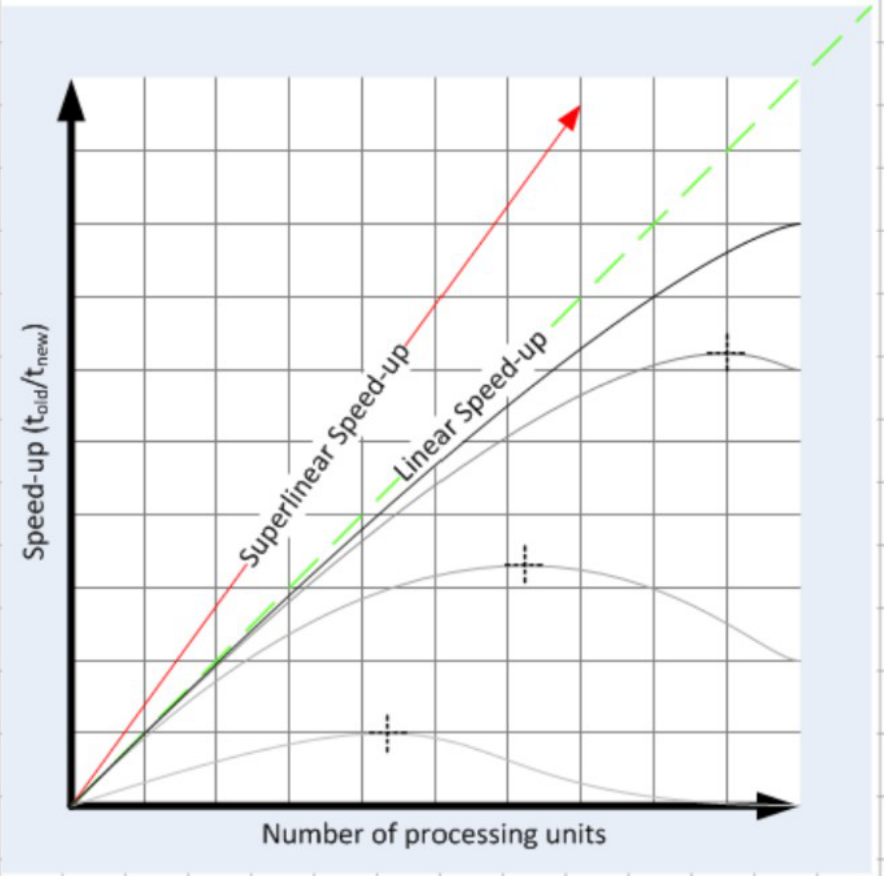
\includegraphics[width=0.46\textwidth]{lecture1_speedup_regimes.png}
  \caption{Speedup regimes as the number of processing units increases.}
  \label{fig:speedup}
\end{figure}

\subsection{Parallel efficiency}
Efficiency measures the speedup obtained per processing unit:
\begin{equation}
  \boxed{E(N)=\frac{S(N)}{N}=\frac{T_1(M)}{N\,T_N(M)}.}
\end{equation}
Linear speedup gives $E(N)=1$; sublinear speedup gives $E(N)<1$.
Superlinear speedup gives $E(N)>1$, which is possible when the parallel run
benefits from architectural effects absent from the sequential baseline.
Efficiency is a relative performance metric, not a direct measurement of
processor utilization.

\newpage
\section{Amdahl's law}
\subsection{Assumptions and derivation}
Amdahl's law describes the speedup of a fixed workload when only part of
its original execution time can be accelerated. Let
\begin{itemize}
  \item $T_1$ be the original sequential execution time;
  \item $p$ be the parallelizable fraction of that time;
  \item $s=1-p$ be the serial fraction;
  \item $N$ be the number of processing units.
\end{itemize}
The ideal parallel model assumes unchanged serial work, perfect load balancing,
no parallel overhead, and an $N$-fold acceleration of the parallel portion.
The execution time is the \textbf{sum} of the serial and parallel contributions:
\begin{align}
  T_{\mathrm{serial}}&=(1-p)T_1,\\
  T_{\mathrm{parallel}}&=\frac{pT_1}{N},\\
  T_N&=T_1\left((1-p)+\frac{p}{N}\right).
\end{align}
Dividing the original time by the new time gives
\begin{equation}
  \boxed{S(N)=\frac{T_1}{T_N}
        =\frac{1}{(1-p)+p/N}
        =\frac{1}{s+p/N}.}
  \label{eq:amdahl}
\end{equation}
For normalized original time $T_1=1$, the new time is simply
$(1-p)+p/N$. The fractions refer to \emph{execution time}, not to the
fraction of source-code lines that can be parallelized.

\subsection{Limits and diminishing returns}
For $0\leq p<1$, the serial part imposes the limit
\begin{equation}
  \boxed{\lim_{N\to\infty}S(N)=\frac{1}{1-p}=\frac{1}{s}.}
\end{equation}
For example, one hour of serial setup and nine hours of parallelizable work
give $s=0.1$, so the maximum ideal speedup is $10$, regardless of how many
processors are available.

For fixed $0<p<1$, adding processors increases ideal speedup with diminishing
returns. If $p=0$, there is no speedup; if $p=1$, the ideal result is $S(N)=N$.
Under this model, efficiency is
\[
  E(N)=\frac{1}{N(1-p)+p}.
\]
When a serial fraction remains, efficiency decreases as $N$ grows.

\subsection{General form: accelerating any portion}
The same argument applies beyond parallel computing. If a fraction $f$ of
the original time is accelerated by a factor $k$, then
\[
  T_{\mathrm{new}}=T_{\mathrm{old}}\left((1-f)+\frac{f}{k}\right),
  \qquad A(k)=\frac{1}{(1-f)+f/k}.
\]
The parallel form follows by setting $f=p$ and $k=N$.

\newpage
\section{Interpreting results in real applications}
Amdahl's time decomposition is correct under its assumptions. The usual
prediction with an $N$-fold acceleration of the parallel part is idealized:
real execution can be either slower or faster than that prediction.

\subsection{Why the prediction can be too optimistic}
Parallel execution introduces communication, synchronization, thread creation,
scheduling, and load-imbalance costs. A more realistic time model is
\begin{equation}
  T_N=T_1\left((1-p)+\frac{p}{N}\right)+T_{\mathrm{overhead}}(N).
\end{equation}
With positive overhead, the actual speedup is below the ideal prediction.
For example, a computation with an ideal $100\times$ speedup can achieve
less if processors spend substantial time exchanging intermediate results
over a network. At sufficiently large processor counts, increasing communication
costs can even make adding processors counterproductive.

\subsection{Why the prediction can be too pessimistic}
Partitioning data can change the memory behavior. A working set that does
not fit in one processor's cache may fit into the combined caches of several
processors. Fewer slow memory accesses can accelerate the parallel portion
by more than $N$, producing a larger speedup than Equation~\eqref{eq:amdahl}
predicts and potentially even superlinear speedup.

This does not invalidate the decomposition of execution time. It means that
the assumed acceleration of the improved portion must reflect the actual
hardware behavior rather than simply being set equal to $N$.

\subsection{Fixed versus growing workloads}
\textbf{Strong scaling} asks how the execution time changes when the processor
count increases while the total problem size stays fixed. This is the setting
of the parallel Amdahl model.

\textbf{Weak scaling} increases total work with processor count, keeping the
work per processor approximately fixed, and examines how execution time changes.
For example, a weather simulation can use more processors to increase grid
resolution rather than to finish the same simulation sooner.

A related fixed-time question asks how much larger a problem can be solved
in the same elapsed time. Gustafson's law describes scaled speedup using
the serial fraction measured in a parallel run. Its serial fraction need
not equal the fraction measured in the original fixed-size sequential run.
These workload comparisons do not contradict Amdahl's fixed-workload limit.

\subsection{Practical interpretation}
Before comparing speedups, check that the workload and sequential baseline
are comparable, identify communication and synchronization costs, and consider
whether cache behavior changes. A processor count alone is insufficient to
predict application performance.

\newpage
\section{Worked examples and revision}
\subsection{Case A: \texorpdfstring{$p=0.5$, $N=4$}{p=0.5, N=4}}
\[
  \frac{T_4}{T_1}=0.5+\frac{0.5}{4}=0.625,
  \qquad S_A=\frac{1}{0.625}=\boxed{1.6}.
\]
Efficiency is $E_A=1.6/4=0.4=40\%$, and the asymptotic speedup limit is $2$.

\subsection{Case B: \texorpdfstring{$p=0.2$, $N=8$}{p=0.2, N=8}}
\[
  \frac{T_8}{T_1}=0.8+\frac{0.2}{8}=0.825,
  \qquad S_B=\frac{1}{0.825}=\boxed{\frac{40}{33}\approx1.212}.
\]
Efficiency is $E_B=S_B/8=5/33\approx15.15\%$, and the asymptotic limit is $1.25$.

\subsection{What the comparison shows}
Case A has a larger speedup despite using fewer processors, because a larger
fraction of its original time can be parallelized. Case B is dominated by
its $80\%$ serial fraction. Since both $p$ and $N$ change, these cases do not
isolate the effect of processor count.

Keeping $p=0.5$ and changing only $N$ from four to eight instead gives
\[
  S(8)=\frac{1}{0.5+0.5/8}=\frac{16}{9}\approx1.778>1.6.
\]
More processors help for this fixed $p$, but the improvement is limited by
the same serial bottleneck.

\subsection{Key formulas}
\begin{center}
\begin{tabular}{@{}ll@{}}
\toprule
Quantity & Formula\\
\midrule
Measured speedup & $S(N)=T_1/T_N$\\[0.4em]
Parallel efficiency & $E(N)=S(N)/N$\\[0.4em]
Ideal parallel time & $T_N=T_1\bigl((1-p)+p/N\bigr)$\\[0.4em]
Amdahl speedup & $S(N)=1/\bigl((1-p)+p/N\bigr)$\\[0.4em]
Serial-fraction limit & $S_{\max}=1/(1-p)$, for $p<1$\\
\bottomrule
\end{tabular}
\end{center}

\subsection{Checks to remember}
\begin{itemize}
  \item Add the serial and parallel execution times; do not multiply them.
  \item Distinguish the speedup of one portion from the overall speedup.
  \item Check whether the problem size is fixed before applying an Amdahl limit.
  \item State the voltage assumption before using a cubic frequency--power relation.
  \item Explain superlinear speedup through changes in execution behavior,
        such as cache effects, rather than treating it as impossible.
\end{itemize}

\end{document}
